\chapter{Stato dell'arte}
In questo capitolo andrò a definire quali siano i presupposti teorici di alcune delle tecnologie che ho impiegato all'interno del progetto.



%%%%%%%%%%%%%%%%%%%%%%%%%%%%%
\section{Ingegneria del software}
%%%%%%%%%%%%%%%%%%%%%%%%%%%%%
L'ingegneria del software, disciplina nata negli anni '50, ha visto la sua importanza crescere con il tempo. Basti pensare che, secondo lo studio demografico riportato da DAXX\cite{SoftwareEngineersNumbers}, nel 2021 erano al lavoro 26.9 milioni di sviluppatori, aumento di 3 milioni rispetto al 2018 (23.9 milioni). Facendo qualche previsione, secondo i dati a disposizione, nell'articolo si arriva alla conclusione che in 8 anni il numero di sviluppatori duplicherà, si stimano circa 45 milioni.
\\
Quelli elencati sopra sono numeri impressionanti che mettono in luce quanto un mercato, che nel 2021 aveva un valore di 429 miliardi di dollari\cite{SoftwareMarketShare}, sia importante. L'ingegneria del software, se applicata con criterio, consente di trasformare un'idea nel miglior prodotto possibile, capace di attrarre clienti e investitori.
\\
Sviluppare buon software, oggi, può essere accomunato con il processo di ricerca di un pozzo di petrolio.\cite{Larman2016} Affinché l'operazione abbia successo è necessario fare una serie di studi preliminari per identificare un pozzo e stimare quanto l'operazione di estrazione potrebbe arrivare a costare. Allo stesso modo qualsiasi progetto segue una serie di fasi che consentono di procedere nell'opera in modo lineare ed efficace.
\\
Adesso darò una panoramica molto rapida di quali sono le macroattività dello sviluppo.
\begin{itemize}
    \item Analisi preliminari: Quando si esegue analisi preliminare si fanno degli studi di realizzabilità del progetto, come le rilevazioni atte a cercare un pozzo di petrolio, è plausibile che, sebbene si tratti di un progetto di grande qualità, questo non sia fattibile poiché si va oltre i limiti di tempo o di budget.
    \item Design della soluzione: Se il progetto viene ritenuto fattibile, sotto tutti i punti di vista, si passa alla fase di design della soluzione, durante la quale si studiano le funzioni richieste e si definisce la soluzione a livello teorico.
    \item Implementazione: Si implementa la soluzione seguendo la documentazione prodotta durante la fase di design.
\end{itemize}
Ciascuna delle attività descritte sopra è composta da una serie di microattività, è necessario decidere quali di queste eseguire durante il processo di sviluppo al fine di fare tutto ciò che è necessario e nulla di più.
Nella sezione successiva metterò a confronto due correnti di pensiero riguardo allo sviluppo software.

%%%%%%%%%%%%%%%%%%%%%%%%%%%%%
\subsection{Sviluppo agile e sviluppo a Cascata}
%%%%%%%%%%%%%%%%%%%%%%%%%%%%%
Il primo processo di sviluppo che si sia mai imposto è quello a Cascata, questo richiede di trattare le macroattività definite sopra come se fossero una serie di passi sequenziali: passare al Design della soluzione significa che le Analisi sono state terminate del tutto con successo. Non è possibile, in alcun caso, passare da una fase all'altra senza aver prima terminato nella sua interezza la fase che la precede.
\\
Il cliente non viene mai incontrato, e non vedrà il progetto fino a che non sarà stato completato. Inutile dire che, andare a costruire una qualsiasi applicazione senza che il cliente possa vederla, dare delle opinioni o proporre nuove funzionalità, porterà a un prodotto che difficilmente incontrerà le sue aspettative. Inoltre, qualora vi fossero modifiche da effettuare, tutto il percorso di sviluppo dovrebbe ripartire da capo per poter adeguare la documentazione ai cambiamenti. Si è stimato che, nel corso di un processo software, il 25\% circa dei requisiti subiscono un cambiamento, per progetti più grandi le percentuali passano ad un valore tra il 35 e il 50 percento.\cite{Larman2016}
\\
Sebbene io abbia ampiamente mostrato come il processo di sviluppo a Cascata sia un processo software inadatto a gestire la produzione di applicazioni commerciali o enterprise, a causa della centralità dei desideri del cliente, questo non significa che il processo sia stato accantonato. Il metodo di sviluppo a Cascata è infatti spesso utilizzato per progettare software \textit{mission critical} che non possono essere rilasciati con problematiche da risolvere. Basti pensare ai sistemi di controllo per le centrali nucleari o software di sicurezza per aeromobili. Una falla in sistemi del genere potrebbe causare una catastrofe.
\\
Un paradigma più adatto all'ambito di sviluppo di applicazioni è quello Agile.
\\
Il paradigma di sviluppo Agile è stato definito con rigore nel 2001, quando un gruppo di ingegneri interessati a nuove metodologie, ha deciso di individuare una serie di punti cardine per la famiglia dei metodi di sviluppo Agili in un \textit{whitepaper} che potesse essere preso come riferimento per progetti futuri. Di seguito sono proposti i principi agili\cite{AgileManifesto} tradotti in italiano in\cite{Larman2016}
\begin{itemize}
    \item La nostra priorità maggiore è soddisfare il cliente attraverso una consegna, fin dall'inizio e continua, di software di valore.
    \item Accogliere il cambiamento dei requisiti, anche nelle fasi avanzate dello sviluppo. I processi agili favoriscono il cambiamento, per il vantaggio competitivo del cliente.
    \item Distribuire frequentemente software funzionante, in intervalli che vanno da un paio di settimane a un paio di mesi, con una preferenza per intervalli temporali più brevi.
    \item Responsabili dell'organizzazione e sviluppatori devono lavorare insieme, giornalmente, per tutta la durata del progetto.
    \item Costruire progetti intorno a persone motivate. Fornire loro l'ambiente e il sostegno di cui hanno bisogno, e a confidare nel fatto che facciano il loro lavoro.
    \item Il metodo più efficiente ed efficace di fornire informazioni all'interno di un team di sviluppo è la comunicazione faccia a faccia.
    \item La misura principale del progresso è il software funzionante.
    \item I processi agili promuovono uno sviluppo sostenibile. Gli sponsor, gli sviluppatori e gli utenti dovrebbero essere in grado di mantenere un'andatura costante all'infinito.
    \item Una continua attenzione alla perfezione tecnica e alla buona progettazione potenziano l'agilità.
    \item La semplicità, intesa come arte di massimizzare la quantità di lavoro fatto, è essenziale.
    \item Le architetture, i requisiti e i progetti migliori provengono da gruppi di lavoro che si auto-organizzano.
    \item A intervalli regolari, il team riflette su come diventare più efficace, per regolare e migliorare il proprio comportamento di conseguenza.
\end{itemize}
Come è possibile capire, anche da una lettura rapida, il paradigma di sviluppo agile è profondamente diverso dal paradigma a Cascata, questo grazie alla centralità che, il cliente e l'idea, hanno in ogni fase dello sviluppo.
\\
Inoltre, l'obiettivo principale del paradigma agile è quello di produrre del codice eseguibile e di valore il prima possibile, in modo che questo possa essere rilasciato, così che anche il pubblico possa provarlo e fare conoscere agli sviluppatori la propria opinione. Le idee del pubblico (soprattutto per i lanci di applicazioni commerciali) influenzano molto il risultato finale, e possono dare dimostrazione di falle che in fase di testing non erano nemmeno state individuate.
\\
A partire da questa definizione sono nati moltissimi metodi di sviluppo agile, come Scrum o 
DevOps\footnote{DevOps è una metodologia di sviluppo del software utilizzata in informatica che punta alla comunicazione, collaborazione e integrazione tra sviluppatori e addetti alle operations della information technology.\cite{DevOpsWiki}},
che differiscono essenzialmente per il modo e il periodo in cui vengono eseguite le attività caratteristiche dello sviluppo.
\\
Adesso passerò ad illustrare brevemente le caratteristiche del metodo di sviluppo agile Scrum.

%%%%%%%%%%%%%%%%%%%%%%%%%%%%%
\subsection{Metodo Scrum}
%%%%%%%%%%%%%%%%%%%%%%%%%%%%%
Scrum è un framework di sviluppo agile che aiuta i team a lavorare insieme. Proprio come una squadra di rugby (a cui deve il nome) che si allena per un grande evento sportivo, il framework Scrum incoraggia i team a imparare attraverso l'esperienza, a organizzarsi in modo autonomo mentre lavorano su un problema e a riflettere sui risultati conseguiti e sugli insuccessi per migliorare continuamente.\cite{ScrumAtlassian}
\\
Quando si applica Scrum il processo di sviluppo viene diviso in sprint\footnote{Uno sprint è un periodo di durata fissa, da una settimana a qualche mese al massimo. La lunghezza del periodo è definita all'inizio del processo e dipende da molti fattori come: la complessità del progetto, il numero di persone che lavorano e la frequenza degli aggiornamenti desiderati dal cliente}. Le feature di interesse che devono essere implementate nel progetto vengono inserite in un product backlog (solitamente visualizzato in forma tabellare) ordinato per importanza.
\\
Il team si incontra ogni giorno, solitamente la mattina, per poter capire quali sono gli obiettivi futuri e cosa è già stato completato da ognuno. L'obiettivo di queste riunioni è quello di condividere i propri problemi e i propri successi di modo che tutto il gruppo possa aiutare e giovarne. Al termine dello sprint c'è invece una fase di revisione con il Product Owner\footnote{Il cliente} chiamata Sprint Review, durante la quale si mostrano al cliente le nuove funzioni implementate e si discute delle possibilità del prossimo sprint.\cite{Larman2016}
\\
Al team Scrum sono associate una serie di figure che consentono al gruppo di funzionare correttamente, l'obiettivo sarebbe quello di isolare il team dalle richieste del cliente, che è la principale causa di cambiamenti nei requisiti del progetto; così che gli sviluppatori si possano concentrare sugli obiettivi che sono stati fissati per lo sprint.
Il Product Owner si interfaccia con lo Scrum Master, che è una figura di riferimento per tutto il team di sviluppo in quanto:
\begin{itemize}
    \item \'E la loro guida,
    \item \'E quello che li protegge dalle influenze del cliente,
    \item \'E colui che spiega le volontà del cliente al team qualora non fossero chiare;
\end{itemize}
Il team è dunque composto da tutte le figure che si occupano dello sviluppo del software, dallo Scrum Master e dal Product Owner.



%%%%%%%%%%%%%%%%%%%%%%%%%%%%%
\section{Microservizi}
%%%%%%%%%%%%%%%%%%%%%%%%%%%%%
In questa sezione spiegherò cosa siano i microservizi e a cosa debbano la grande popolarità che stanno acquisendo.

%%%%%%%%%%%%%%%%%%%%%%%%%%%%%
\subsection{Progetto Monolita e Progetto a Microservizi}
%%%%%%%%%%%%%%%%%%%%%%%%%%%%%
Quando ci si approccia al mondo dell'informatica, da un punto di vista scolastico, si impara a strutturare un applicativo in modo tale da avere un main e una serie di elementi che sono ad esso collegati\footnote{Affermazione che dipende dal tipo di paradigma di programmazione impiegato}. Fin da subito, dunque, ci viene insegnato un approccio monolitico allo sviluppo del software. Pertanto i primi progetti sviluppati in ambito didattico sono, essenzialmente, dei blocchi che contengono tutto il necessario per far funzionare l'applicazione correttamente.
\\
Contrapposto allo sviluppo monolitico, c'è lo sviluppo a microservizi. La differenza essenziale tra le due visioni è che, mentre lo sviluppo monolitico comprime tutte le funzionalità all'interno di un'unica unità, il progetto a microservizi le spezza in una serie di componenti indipendenti. In seguito passerò ad analizzare quali siano i punti di forza e le debolezze di ciascuno stile architetturale. Prima però passo a esplorare più nel dettaglio perché compagnie come: Netflix, Uber e Sound Cloud; per citarne qualcuna, hanno scelto di sviluppare i propri applicativi web a microservizi.
\\
I microservizi sono una tecnica di sviluppo tramite la quale viene prodotto del software composto da  servizi indipendenti, di piccole dimensioni, che comunicano tra loro tramite API ben definite. Questi servizi sono controllati da team autonomi. Le architetture dei microservizi permettono di scalare e sviluppare le applicazioni in modo più rapido e semplice, permettendo di promuovere l’innovazione e accelerare il time-to-market di nuove funzionalità.\cite{MicroserviceAmazon}
\\
Lavorare frammentando l'intero team in sub-team indipendenti più piccoli, che lavorano ciascuno su una funzionalità dell'applicativo come se fossero progetti autonomi, consente di aumentare la produttività e di costruire progetti più grandi più facilmente. Questo perchè è stato "spazzato sotto il tappeto" il problema di comporre i prodotti dello sviluppo dei vari team.
\\
Se i team sono stati costruiti bene, e le funzionalità sono state distribuite correttamente, ciascuno sarà capace di lavorare per conto proprio, senza dover comunicare con gli altri, tranne i casi in cui vi dovesse essere comunicazione tra i vari microservizi. La diminuzione degli scambi di informazioni tra team diversi riduce le incomprensioni, inoltre, essendo i gruppi indipendenti e autogestiti, possono seguire un proprio stile di programmazione e possono impiegare le tecnologie che più si adattano alla risoluzione del problema loro assegnato.
\\
Esattamente come nel caso della scelta del processo di sviluppo (Cascata o agile), anche in questo caso c'è la possibilità di scegliere se impiegare un'architettura a microservizi o impiegarne una monolitica. Come dicevo in precedenza, le due tecniche hanno dei pregi e dei difetti che ho riassunto in due tabelle distinte, tali valutazioni sono state prese da \cite{ProsConsMicroservices}.
\\
Parto con i punti di forza dei due stili architetturali.

\begin{center}
    \begin{tabular}{|p{0.45\linewidth}|p{0.45\linewidth}|}
    \hline
    \textbf{Microservices} & \textbf{Monolith}\\
    \hline
    \rowcolor{LighterGreen}
     La struttura a microservizi è estremamente \textbf{flessibile}, qualsiasi problema rimane isolato a un unico servizio o a un piccolo gruppo. &  Il sistema monolitico è \textbf{semplice da controllare}, non ci sono elementi multipli da considerare dunque operazioni come logging, caching e performance analysis sono semplici da eseguire.\\
    \hline
    \rowcolor{Green}
     La struttura a microservizi è più \textbf{semplice da comprendere} (in particolare il singolo microservizio) visto che non è costituita da un unico progetto enorme. & Il sistema monolitico può essere \textbf{testato e debuggato con facilità}. \\
    \hline
    \rowcolor{LightGreen}
    La struttura a microservizi può \textbf{scalare} con maggiore facilità. & Il sistema monolitico è \textbf{semplice da deployare}. \\
    \hline
    \rowcolor{LighterGreen}
    & Il sistema monolitico è \textbf{semplice da sviluppare}. \\
    \hline
    \end{tabular}
\end{center}

Passo ora alle debolezze

\begin{center}
    \begin{tabular}{|p{0.45\linewidth}|p{0.45\linewidth}|}
    \hline
    \textbf{Microservices} & \textbf{Monolith}\\
    \hline
    \rowcolor{Red}
     La struttura a microservizi è un sistema distribuito complesso che richiede \textbf{conoscenze specifiche} da parte di chi lo gestisce. &  Il sistema monolitico è \textbf{difficilmente scalabile} in quanto deve scalare l'intera applicazione, non è possibile farne scalare solo una parte. \\
    \hline
    \rowcolor{LightRed}
     Gestire lo \textbf{stato} di una struttura a microservizi è più complesso dato che ogni servizio è indipendente dagli altri. & Il sistema monolitico viene \textbf{aggiornato con maggiore difficoltà}, soprattutto qualora gli elementi che lo compongono dovessero essere altamente accoppiati. \\
    \hline
    \rowcolor{LightRed}
    La struttura a microservizi è \textbf{difficile da testare}. & Cambiare una delle tecnologie impiegate in un progetto monolitico significa che è necessario \textbf{riscriverlo da capo}\footnote{
    Sebbene l'affermazione abbia un che di sensazionalistico, cambiare una tecnologia all'interno di un progetto monolitico può significare, veramente, la riscrittura di buona parte del codice.
    }. \\
    \hline
    \end{tabular}
\end{center}

Ciò detto, non si può arrivare a proclamare un vincitore tra sviluppo a microservizi e sviluppo monolitico, perchè non si tratta di una competizione. Si potrebbe affermare che, ragionando in ambito enterprise, la soluzione a microservizi sia migliore sul lungo periodo rispetto al sistema monolitico, se guardiamo però la figura \ref{fig:complexity}\footnote{L'immagine è stata presa da \cite{MartinFowlerDotCom}} possiamo vedere come la risposta alla domanda "che tipo di architettura dovrei impiegare?" è dipende.

\begin{figure}[h]
    \centering
    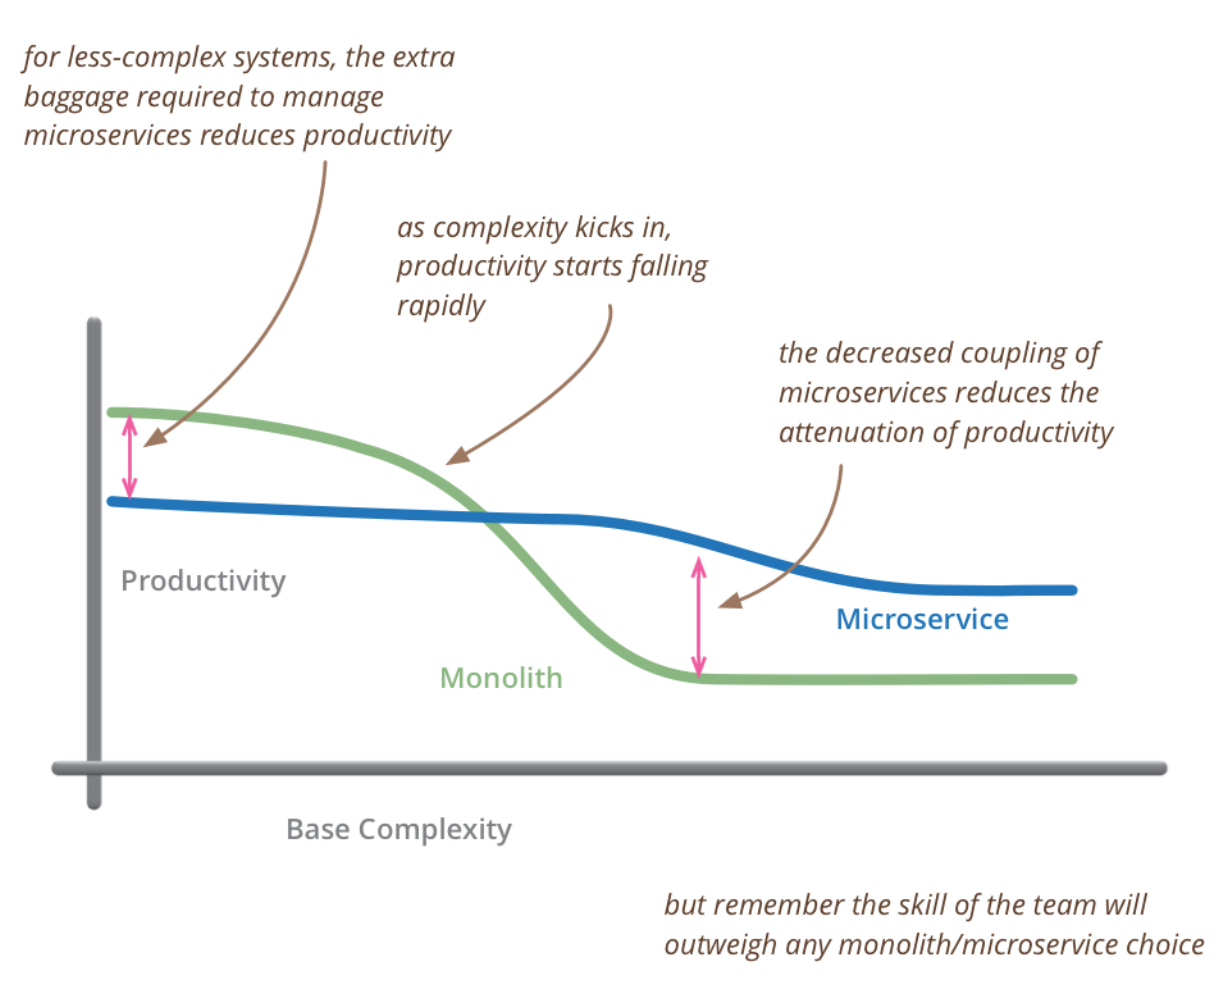
\includegraphics[width=450px]{./images/microserviceComplexity.png}
    \caption{Grafico che raffronta la produttività al tipo di architettura software impiegato}
    \label{fig:complexity}
\end{figure}

Come mostrato nel grafico \ref{fig:complexity} se il progetto non è complesso non ha senso costringere il team a scontrarsi con le difficoltà aggiunte dei microservizi, soprattutto qualora il prodotto dovesse cambiare raramente. All'aumentare della complessità l'architettura a microservizi è invece una scelta sostanzialmente automatica perchè (come evidenziato nelle tabelle precedenti), l'elevato accoppiamento degli elementi di un progetto monolitico rende ogni modifica e ogni problema più difficile da risolvere.
\\
Nella sezione seguente spiegherò come possano essere composti dei servizi all'interno dell'architettura a microservizi.

%%%%%%%%%%%%%%%%%%%%%%%%%%%%%
\subsection{Orchestrazione e Coreografia}
%%%%%%%%%%%%%%%%%%%%%%%%%%%%%
Quando si esegue la composizione di microservizi ci sono due strutture diverse su cui si può fare affidamento, la struttura Orchestrata è una struttura che fa capo a un "maestro" e, come suggerisce il nome, l'obiettivo è quello di simulare un'orchestra. Ogni singolo microservizio non "conosce" il proprio ruolo e il proprio posto, quindi è compito del maestro far sapere ai componenti quand'è il momento di entrare in azione.
\\
Per tradurre il concetto in modo più formale, si può utilizzare un orchestratore che si occupa di gestire le comunicazioni tra i microservizi poiché conosce le API di comunicazione che vengono utilizzate e conosce l'ordine secondo cui devono essere chiamati i servizi per poter completare la richiesta. I microservizi non sono a conoscenza del flusso generale delle informazioni ma solo della parte che è di loro dominio. \cite{AzureCloudPatterns}

\begin{figure}[h]
    \centering
    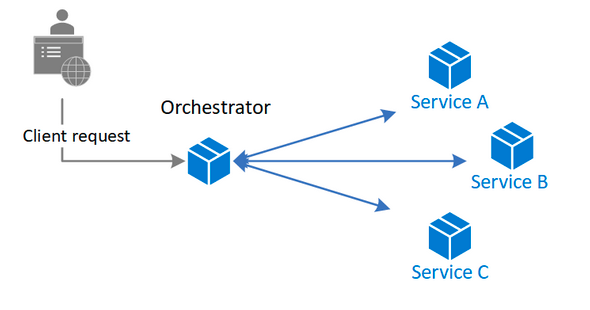
\includegraphics[width=300px, height=130px]{./images/orchestration.png}
    \caption{Un diagramma che illustra un esempio di sistema orchestrato}
    \label{fig:orchestration}
\end{figure}

Avere una figura centrale che si occupa di gestire le comunicazioni tra i vari microservizi aggiunge un overhead che spesso può essere d'intralcio, quindi si potrebbe tendere verso una rappresentazione alternativa, che è quella coreografata. In questo caso tutti i microservizi sono indipendenti e sono in grado di comunicare con i servizi che sono loro necessari per poter portare avanti la transazione senza bisogno di un'entità super partes che coordini le operazioni.

\begin{figure}[h]
    \centering
    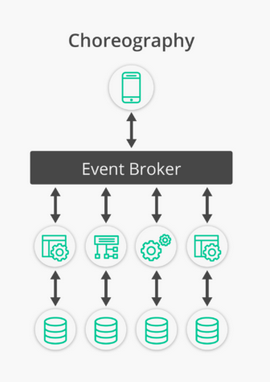
\includegraphics[height=200px]{./images/choreography.png}
    \caption{Un diagramma che illustra un esempio di sistema coreografato}
    \label{fig:coreography}
\end{figure}

Quando si dovrebbe prediligere la coreografia all'orchestrazione?
\\
Quando ci si aspetta che l'applicativo verrà cambiato spesso, in particolare quando è previsto che verranno aggiunti e tolti servizi di frequente. La struttura coreografata consente di apportare tali modifiche abbastanza facilmente e soprattutto creando la minima quantità di \textit{disruption} per i servizi che rimangono attivi.\cite{AzureCloudPatterns} Inoltre una struttura coreografata consente di rimuovere l'overhead che caratterizza l'orchestratore.
\\
Quand'è che invece vale il vice versa?
Sebbene le infrastrutture orchestrate abbiano un unico punto di fallimento, l'orchestratore, che le rende meno resilienti, sono più semplici da gestire, ed è più semplice recuperare dopo gli errori. Inoltre è più semplice parallelizzare e far scalare un'architettura orchestrata. Se il numero di componenti cresce troppo velocemente, diventa difficile gestire una struttura coreografata, a causa del grande numero di elementi indipendenti.\cite{AzureCloudPatterns}
\\
Ora, per concludere la sezione sull'ambito dei microservizi vorrei passare alla differenza fondamentale che c'è tra una Virtual Machine (tipo quelle che vengono utilizzate da VirtualBox) e un container, contenitori virtuali utilizzati da software come Docker. 

%%%%%%%%%%%%%%%%%%%%%%%%%%%%%
\subsection{Container e Virtual Machine}
%%%%%%%%%%%%%%%%%%%%%%%%%%%%%
Un container Docker è un pacchetto leggero, \emph{standalone} ed eseguibile che include tutto ciò che è necessario per eseguire l'applicazione.\cite{Containers} La struttura di un gruppo di applicazioni containerizzate è mostrata nella figura \ref{fig:containerStructure}

\begin{figure}[h]
    \centering
    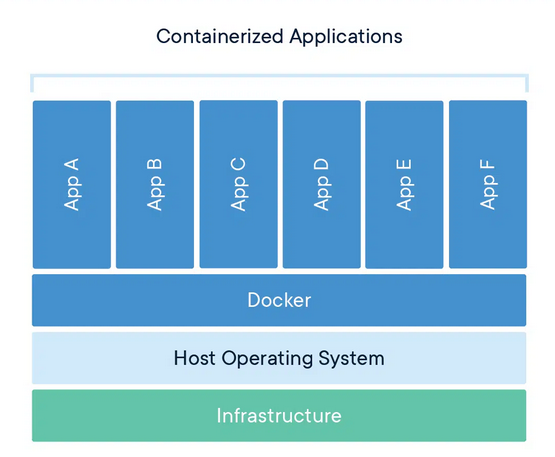
\includegraphics[height=200px]{./images/docker_container.png}
    \caption{Uno schema che mostra come un ambiente Docker possa girare sopra un sistema operativo}
    \label{fig:containerStructure}
\end{figure}

Come si può vedere vi sono una serie di container indipendenti gli uni dagli altri che girano al di sopra dell'engine Docker.
\\
Contrariamente ai container, un ambiente virtualizzato, è un componente standalone che gira su un layer di virtualizzazione che si interfaccia con l'hardware. Una virtual machine contiene al suo interno un sistema operativo ospite nella sua interezza e questo le rende più lente rispetto ai container. \'E possibile vedere la struttura di un ambiente virtualizzato nella figura \ref{fig:virtualMachine}.

\begin{figure}[h]
    \centering
    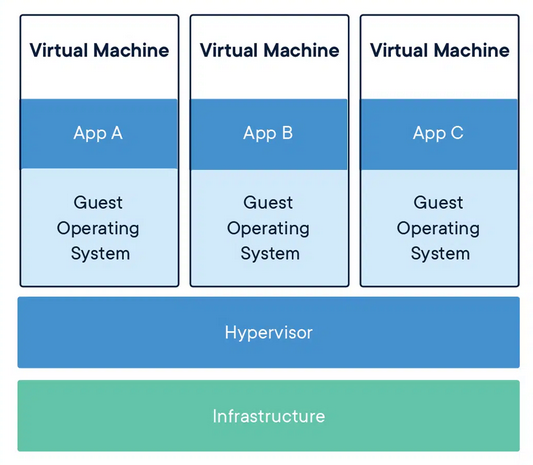
\includegraphics[height=200px]{./images/virtualization.png}
    \caption{Un diagramma che illustra la struttura di una virtual machine}
    \label{fig:virtualMachine}
\end{figure}

Di seguito riporto qualche dato, riguardo alla dimensione media di una Virtual Machine, ricavato dalle linee guida di Virtual Box.\footnote{
VirtualBox è un prodotto di virtualizzazione x86 AMD64/Intel64 per ambito enterprise e privato. VirtualBox non è solo feature-rich e ad elevate prestazioni, adatto ai clienti enterprise, si tratta anche dell'unica soluzione professionale che sia disponibile gratuitamente come software Open Source secondo i termini del GPL versione 2.\cite{VirtualBox}
} Secondo la guida, la dimensione che una virtual machine può arrivare ad occupare, è di qualche decina di GB\cite{VirtualBoxGuideLines} (ovviamente ciò dipende dal sistema operativo che è stato montato sulla macchina virtuale). Per quanto riguarda le dimensioni tipiche di un container, non sono riuscito a trovare dati rilevanti, a parte qualche risposta su forum specializzati e un articolo derisorio intitolato \textit{How to Not Be the Engineer Running 3.5GB Docker Images}\cite{SarcasticArticle}, è evidente come, a discapito di quello che si dice di solito, le dimensioni contino eccome.
\\
\'E vero a tal punto che si utilizzano, per quel che riguarda le immagini Docker, i processi di build in due fasi, al fine di ridurre al minimo le dimensioni dei container.
\\
Si supponga di voler creare un container per ReactJS, per poterlo fare dobbiamo importare un'immagine Node che consenta di eseguire il processo di build del progetto. Una volta che questo è terminato, però, i file di Node risultano di fatto inutili. Quindi si potrebbe impiegare un processo di build in due fasi per rendere il progetto React eseguibile e poi caricare nel container solo i file necessari, tralasciando tutto ciò che è Node.
\\
Indipendentemente da quanto detto sopra è ovvio che, come nella maggior parte dei casi nel mondo informatico, ogni tecnologia ha un suo motivo di essere. Mettere a confronto le dimensioni di Container e Macchine virtuali non ha alcuno scopo, se non mettere in luce il fatto che i container vengono normalmente impiegati al posto delle virtual machine in ambiti come Docker e la creazione di cluster Kubernetes perchè sono soluzioni veloci e light-weight.



%%%%%%%%%%%%%%%%%%%%%%%%%%%%%
\section{API Rest}
%%%%%%%%%%%%%%%%%%%%%%%%%%%%%
Un'API REST, nota anche come API RESTful, è un'interfaccia di programmazione delle applicazioni (API o API web) conforme ai vincoli dello stile architetturale REST, che consente l'interazione con servizi web RESTful. Il termine REST, coniato dall'informatico Roy Fielding, è l'acronimo di REpresentational State Transfer.\cite{APIRest}
\\
REST è un insieme di vincoli architetturali, né un protocollo né uno standard, chi sviluppa API può decidere se implementare tutti i vincoli di REST, producendo dunque un'API RESTful, oppure implementarne solo alcuni. I vincoli architetturali sono i seguenti:
\begin{itemize}
    \item Lo stato dell'applicazione e le funzionalità sono divisi in risorse web
    \item Ogni risorsa è unica e indirizzabile
    \item tutte le risorse sono condivise come interfaccia uniforme per il trasferimento di stato tra client e risorse, questo consiste in.
        \begin{itemize}
            \item Un insieme vincolato di operazioni ben definite.
            \item Un insieme vincolato di contenuti, opzionalmente supportato da codice a richiesta
            \item Un protocollo che è:
            \begin{itemize}
                \item client-server
                \item stateless\footnote{
                Una comunicazione è stateless quando non viene tenuta in memoria alcuna traccia delle transazioni passate. Dunque ogni singolo messaggio della comunicazione deve essere self-explanatory
                }
                \item Memorizzabile in cache
                \item A livelli
            \end{itemize}
        \end{itemize}
\end{itemize}
Le API REST hanno un gran numero di vincoli che però servono a renderle leggere e veloci, infatti questo modello ha sradicato il modello SOAP\footnote{Simple Object Access Protocol} basato su messaggi e requisiti XML che lo rendevano complesso e pesante.\cite{APIRest}
\\
Secondo Roy Fielding l'applicazione delle regole previste dai vincoli consentono di costruire un'applicazione che sia facilmente scalabile, nella sua dissertazione l'ideatore di REST lega la scalabilità delle applicazioni web ai vincoli architetturali in questo modo\cite{Fielding2000}:

\begin{displayquote}
La separazione REST client-server degli interessi semplifica l'implementazione del componente, riduce la complessità della semantica del connettore, migliora l'efficacia dell'ottimizzazione delle prestazioni ed aumenta la scalabilità di componenti server puri. I vincoli di sistema a strati permettono di introdurre intermediari — proxy, gateway, e firewall — in vari punti della comunicazione senza cambiare le interfacce tra i componenti, consentendo loro di assistere nella traduzione della comunicazione o migliorare le prestazioni tramite cache condivisa di larga scala. REST consente l'elaborazione intermedia vincolando i messaggi ad essere auto-descrittivi: l'interazione è priva di stato tra le richieste, i metodi di base ed i tipi di media sono utilizzati per indicare la semantica e scambiare informazioni e le risposte indicano esplicitamente la possibilità di memorizzare nella cache.\footnote{
Ho trovato la citazione tradotta su Wikipedia \cite{RESTWikipedia}
}
\end{displayquote}

Passerò ora a dare qualche definizione di base in ambito di sicurezza.

%%%%%%%%%%%%%%%%%%%%%%%%%%%%%
\section{Ambito di sicurezza}
%%%%%%%%%%%%%%%%%%%%%%%%%%%%%
Sebbene non si trattasse prettamente del mio ambito penso sia utile considerare rapidamente quali siano le logiche di sicurezza più comuni nel campo delle comunicazioni.
\\
In questa sezione esplorerò i seguenti concetti:
\begin{itemize}
    \item Cifratura a chiave segreta
    \item Cifratura a chiave pubblica
\end{itemize}
Ai fini della mia applicazione, soprattutto per quel che riguarda gli sviluppi futuri, la logica di implementazione della chiave pubblica è più importante, però penso sia una buona idea passare prima dalla tecnica a chiave segreta.

%%%%%%%%%%%%%%%%%%%%%%%%%%%%%
\subsection{Cifratura a chiave segreta}
%%%%%%%%%%%%%%%%%%%%%%%%%%%%%
I primi veri passi nell'ambito della protezione dei dati sono stati fatti quando è stato ideato il meccanismo di cifratura a chiave segreta, detta crittografia simmetrica.
\\
Questo meccanismo prevede l'utilizzo di una chiave, condivisa tra due utenti, per poter cifrare e decifrare i messaggi.

\begin{figure}[h]
    \centering
    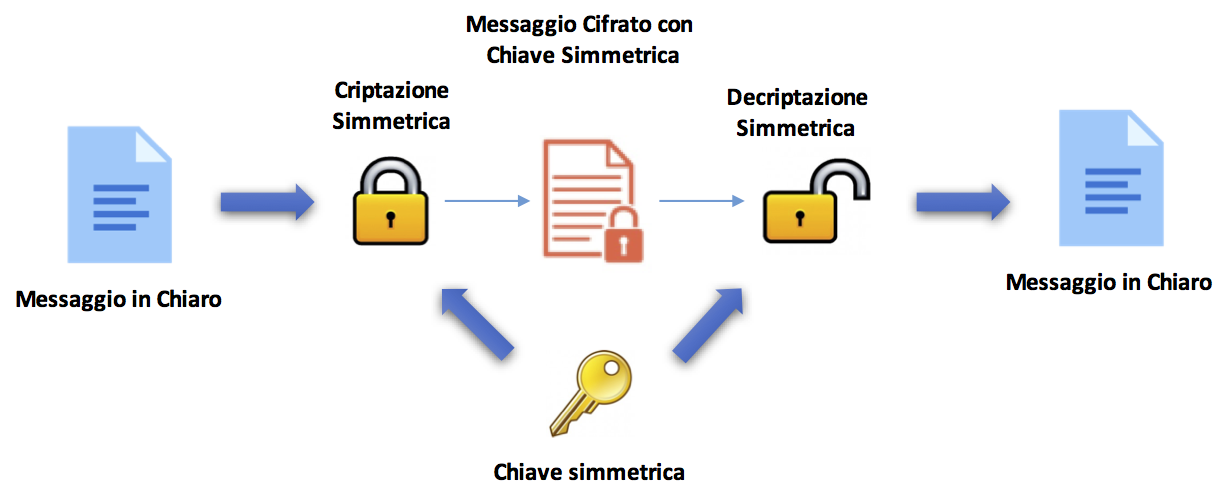
\includegraphics[width=300px]{./images/criptazione_simmetrica.png}
    \caption{Un diagramma che illustra la logica della crittografia simmetrica}
    \label{fig:symmetricalCryptography}
\end{figure}

Questo metodo di cifratura ha una serie di vulnerabilità molto evidenti che lo rendono poco adatto a una buona varietà di contesti.
\\
Anzitutto si tratta di un sistema crittografico che può essere facilmente violato tramite social engineering, la chiave deve rimanere un segreto in un gruppo di persone e, se si eseguono più comunicazioni in parallelo, la difficoltà di mantenere le chiavi effettivamente segrete aumenta. Infatti il numero di chiavi necessarie per comunicare in un gruppo è limitato superiormente da\cite{Anderson2008}:

\begin{equation}
    \frac{n * (n - 1)}{2}
\end{equation}

Sebbene il sistema sia tecnicamente inadatto, come già detto in precedenza, a gestire tutta una serie di situazioni, si tratta di un metodo di cifratura le cui declinazioni (DES\footnote{
DES è un algoritmo di cifratura che sfrutta la crittografia simmetrica, la logica è quella di cifrare un messaggio dividendolo in blocchi da 64 bit ed eseguendo operazioni combinatorie su ciascun blocco a partire da una funzione combinatoria e la chiave segreta della sessione. Il processo viene ripetuto su ogni blocco per 16 volte.
\\
L'algoritmo era stato ideato come standard di sicurezza ed è stato successivamente abbandonato poichè era possibile violarlo utilizzando computer facilmente accessibili alle aziende.
}, AES\footnote{
AES è un algoritmo che è venuto dopo DES e che implementa una logica simile ma su blocchi e chiavi di dimensione diversa, così da renderlo più difficile da violare
}, etc...) possono essere implementate sia livello software che livello hardware di modo che vengano eseguite rapidamente.

%%%%%%%%%%%%%%%%%%%%%%%%%%%%%
\subsection{Cifratura a chiave pubblica}
%%%%%%%%%%%%%%%%%%%%%%%%%%%%%
La cifratura a chiave pubblica, anche detta crittografia asimmetrica seguì un periodo di gestazione di tre anni, infatti Nel 1970, James H. Ellis, crittografo inglese presso il Government Communications Headquarters (GCHQ), immaginò la possibilità di una "crittografia non segreta", ma non riusciva a vedere alcun modo di implementarla. Nel 1973, il suo collega Clifford Cocks realizzò quello che è diventato noto come algoritmo di crittografia RSA, dando un metodo pratico di "cifratura non segreta".\cite{CrittografiaAsimmetricaWiki}
\\
La logica dietro alla crittografia asimmetrica prevede che per ogni individuo che intenda impiegarla, venga generata una coppia di chiavi (chiave pubblica, chiave privata). Il nome di ciascuna chiarisce già il pubblico per cui la chiave è pensata, una deve essere nota solo al possessore, l'altra è destinata a qualsiasi canale pubblico.
\\
Ciò che viene criptato con una chiave può essere decriptato solo con l'altra e vice versa.

\begin{figure}[h]
    \centering
    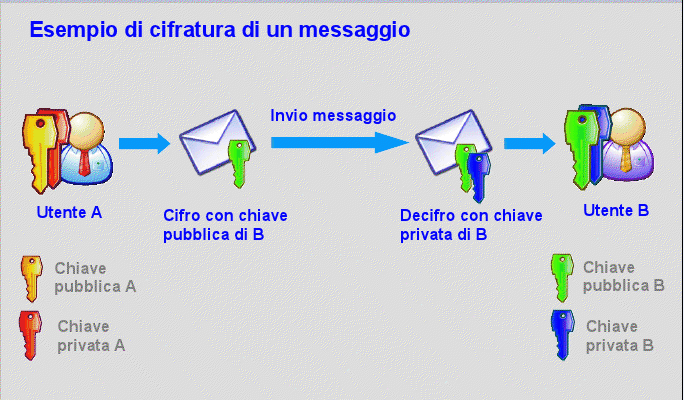
\includegraphics[width=300px, height=160px]{./images/cifratura_messaggio.png}
    \caption{Un diagramma che illustra la logica della crittografia asimmetrica}
    \label{fig:asymmetricalCryptography}
\end{figure}

Oltre alla cifratura di messaggi sensibili, la crittografia asimmetrica può essere impiegata per gestire firme digitali\footnote{
La firma digitale è un metodo matematico teso a dimostrare l'autenticità di un messaggio o di un documento digitale inviato tra mittente e destinatario attraverso un canale di comunicazione non sicuro\cite{FirmaDigitale}
}: l'utente A cifra un messaggio con la propria chiave privata e chiunque, all'interno di una rete, lo può decifrare impiegando la chiave pubblica di A, di fatto riconoscendo che il messaggio poteva essere stato inviato solo ed unicamente da A\footnote{
In questo caso si ignora volutamente il fatto che la chiave privata potrebbe essere stata rubata ad A tramite, per esempio, phishing o social engineering
}.
